%________________________________________
%CaRS Move I "Establish a territory" (Situation):
% * Important area
% * Introducing and reviewing items of previous  research <--(ToDO)
Ship dynamics predictive models have a wide range of applications, e.g., safety enhancements, route planning and optimization, autonomous shipping, etc., \citep{aslam_internet_2020}.
Ship manoeuvring is a sub field of ship dynamics with well established system based models such as: \citet{abkowitz_ship_1964,nomoto_steering_1957,norrbin_theory_1971}, and the MMG model \citep{yasukawa_introduction_2015}.

Captive model tests is the classical approach to identify the parameters within these models. However, this approach is not practically applicable for the full scale ships; Instead, computational fluid dynamics (CFD) with either direct simulations or virtual captive tests (VCT) has emerged as an interesting option for the full scale ship predictions \citep{liu_predictions_2018,li_ship_2022}.
The CFD requires a complete understanding of the system. Acquiring such knowledge may be possible for some cases, but it is not practical in a complex sea environment including: wind, wave and current, with increased modelling uncertainties \citep{miller_ship_2021}; In coastal areas, water depth and the bank effect also add uncertainty  \citep{nielsen_machine_2022};
And even if the sea is flawlessly modelled, long-term predictions with high accuracy will be exposed to deterministic chaos \citep{lorenz_deterministic_1963}.
Together with the other drawbacks of CFD -- such as high computational costs -- data driven models have become an attractive alternative or complement, with an increased number of publications in the past 10-15 years (shown in Fig.\ref{fig:pub_overview}) -- especially within autonomous ships \citep{ahmed_survey_2023}.
%
\begin{figure}[h]
  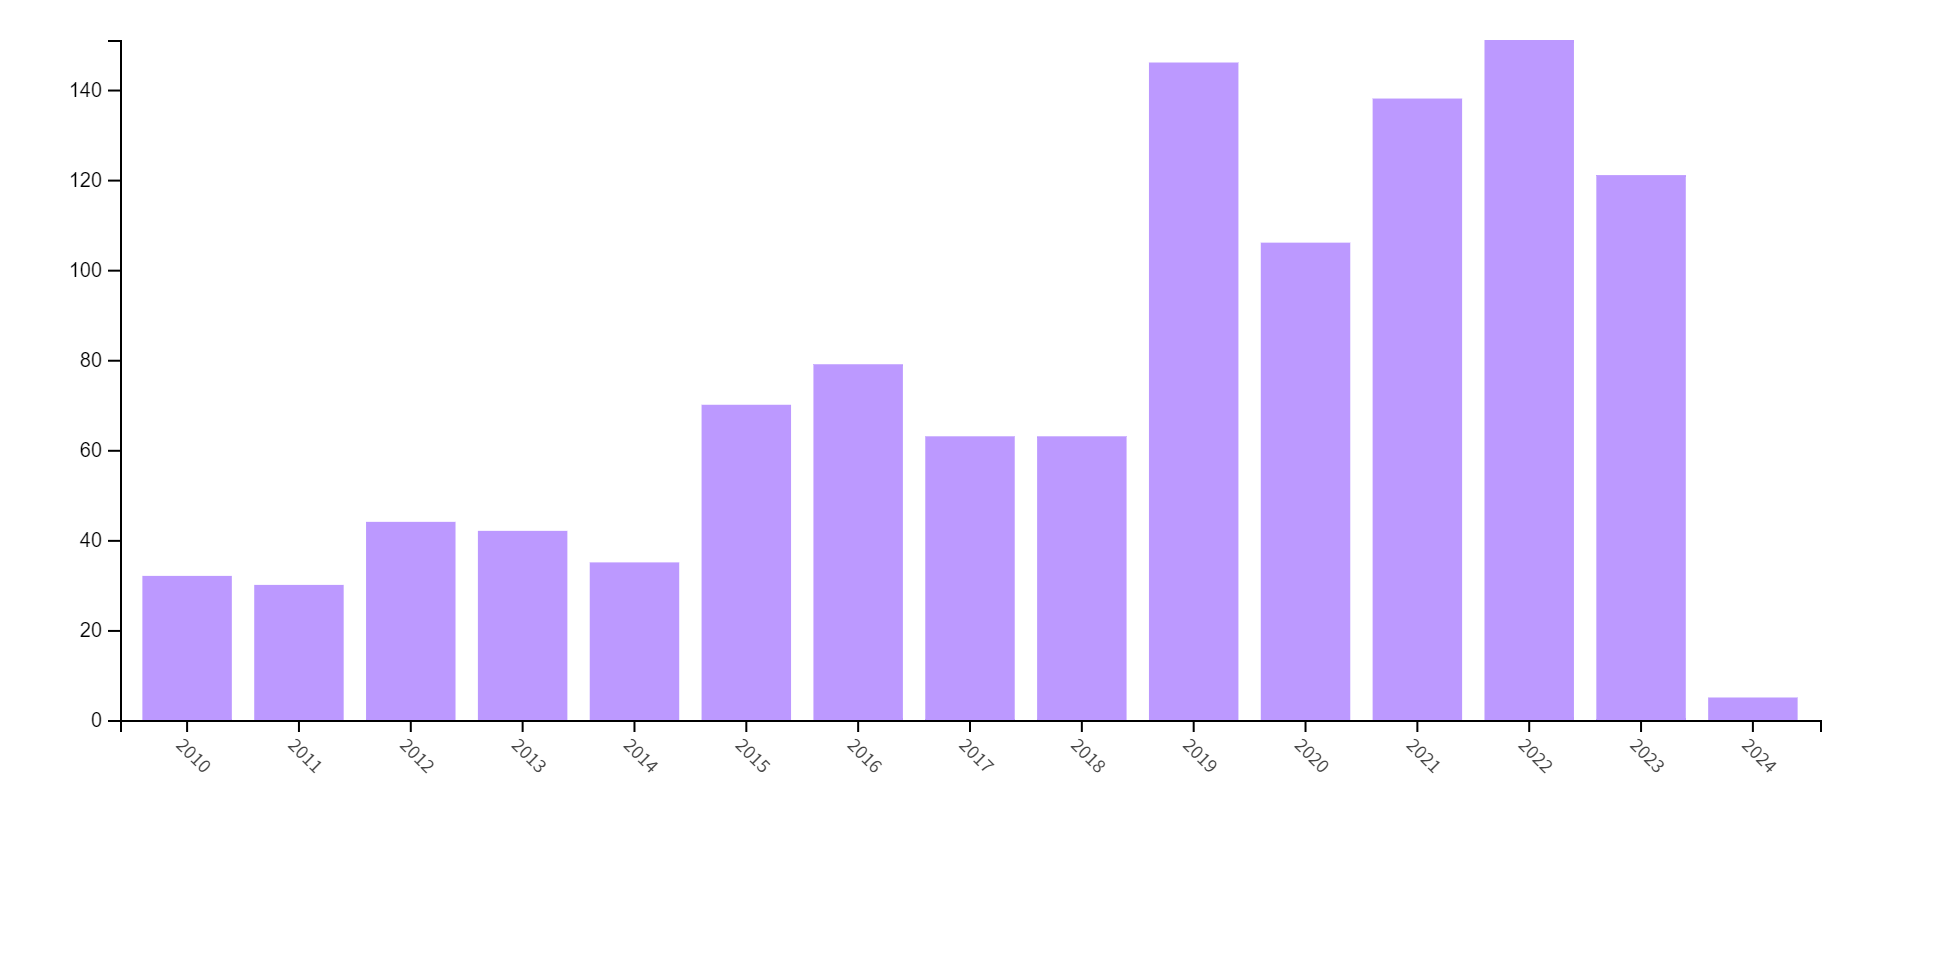
\includegraphics[width=.5\textwidth]{figures/trendinyear.jpg}
  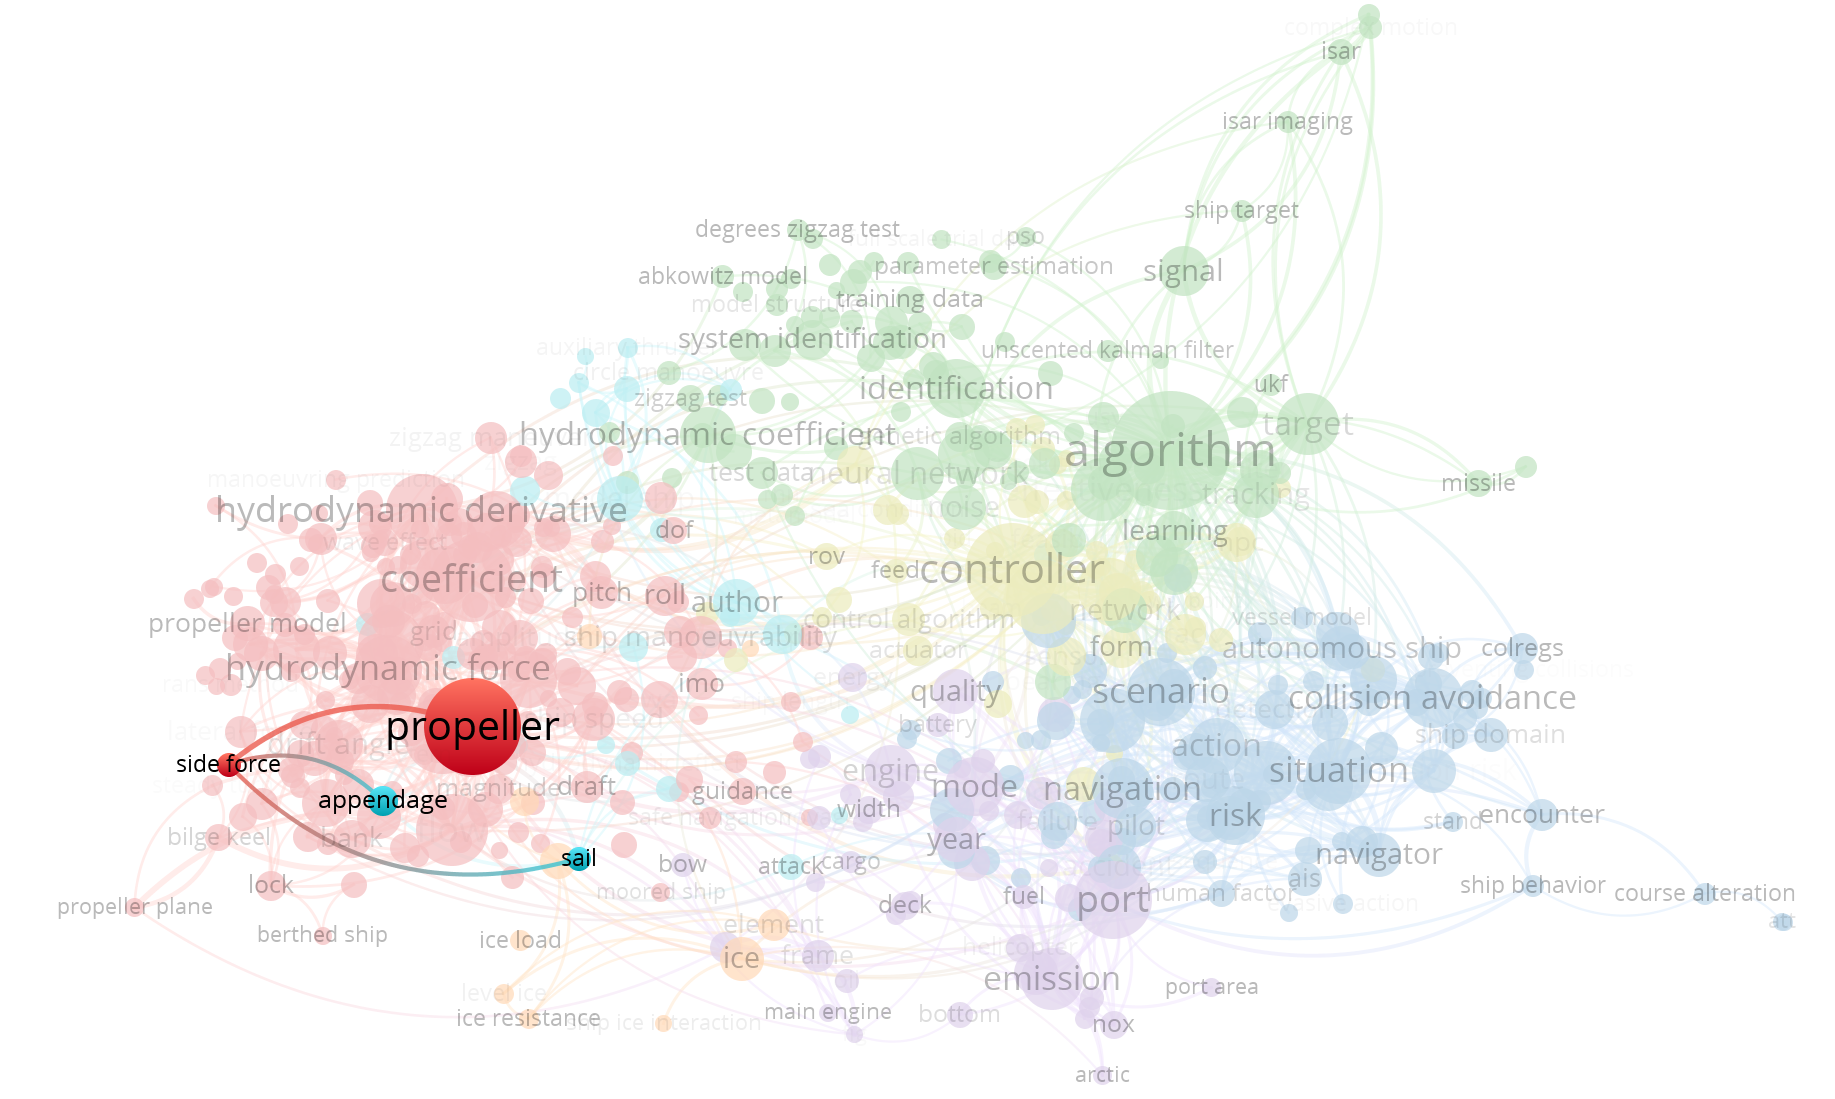
\includegraphics[width=.5\textwidth]{figures/wind_drift_research.png}
  \caption{Research topics within the field of ship maneuverability system identification}
  \label{fig:pub_overview}
\end{figure}
%

Many of these papers have shown that hydrodynamic coefficients can effectively be estimated on simulated data where the exact ''physical'' model is assumed known; However in real cases/applications, the mathematical model is just the simplification of real physics (from VCT, model test, sea trials, or full-scale tests), while the complexity of hydrodynamics involved in vessel maneuvering will greatly challenge the simplified empirical mathematical methods without carefully considering the actual physics inside hydrodynamic coefficients and their interactions. 

One of the earlier papers with real data was proposed in 1976 by \citet{astrom_identification_1976} to develop a linear manoeuvring model that utilized manually recorded data in 1969 aboard the Atlantic Song freighter with Kalman filter (KF) and maximum likelihood estimation. 
The extended Kalman filter (EKF) was used on a nonlinear Nomoto model by \citet{perera_system_2015} and a 3 degree of freedom model by \citet{shi_identification_2009}. The unscented Kalman filter (UKF), which has been proposed as an improvement to the EKF for handling nonlinear systems, was used in \citet{revestido_herrero_two-step_2012}.
Support vector regression (SVR) has been investigated by \citet{luo_parameter_2016}, \citet{zhu_parameter_2017}, and \citet{wang_parameter_2021}. 

%
%________________________________________
%CaRS Move II "Establish a niche" (Problem):
% * counter claim?
% * gap?
% * question       <------
% * continuation?
The input variables of the data-driven ship manoeuvring models are often strongly linearly dependent. This multicollinearity is a well known issue in parameter identification, that may lead to parameter drift and poor generalization; The parameters are thus mathematically correct but physically incorrect \citep{luo_parameter_2016}. 
An example of generalization is when a model identified on calm water data is exposed to wind; A drift angle is now needed to maintain a straight course. This wind state is rare in calm water manoeuvring tests, where the drift angle is almost exclusively accompanied by yaw rate; 
The regression will thus have problems to distinguish between these states.
%
\begin{figure}[h]
    \centering
    \includesvg{figures/multicollineraity.multicollinearity.svg}
    \caption{Phase portrait where the combination of drift angle and yaw rate is shown for zigzag10/10, and zigzag20/20 tests.}
    \label{fig:multicollinearity}
\end{figure}
%

% Wengang fixes a better figure here...
This drifting (side forces) is rarely investigated as shown in Fig.\ref{fig:pub_overview}.

Using more informative data or simplifying the model -- when possible -- and thereby reducing the number of parameters, is one of the most researched ways to mitigate the multicollinearity through some possible remedies such as the difference method \citep{luo_parameter_2016}, principal component analysis (PCA), and partial least squares regression \citep{jian-chuan_parametric_2015}. 

%________________________________________
%CaRS Move III "Occupy the niche" (Solution/Evaluation):
% * outline purpose?
% * list research questions?
% * announce principal findings?            <--
% * stating the value of present research?
% * article structure?                      <--

More remedies are however needed; Therefore, in this paper, a physics informed manoeuvring model, which features a new semi-empirical rudder model based on semi-empirical formulas from the literature, is proposed.

The objective is to identify a model that is not just mathematical correct: but also as physically correct as possible.
To evaluate the physical correctness, two unique datasets from a wind-powered pure car carrier (WPCC) are employed. Data from VCT at various steady-state drift angles, yaw rates, and rudder angles, establish the physically correct kinetics. System identification is conducted via inverse dynamics \citep{faber_inverse_2018} on a second dataset containing a series of manoeuvring model tests with a free model of the WPCC. The identification is conducted for the physics informed model as well as an Abkowitz mathematical manoeuvring model for comparison. The generalization of the models is studied in an idealized wind state.

The left of the paper is organized as follows. The proposed physics informed manoeuvring model is first presented in \autoref{sec:ship_models}, while some mathematical details of the model are given in the appendix. The developed methodology framework to identify parameters within the proposed physics-informed model is described in \autoref{sec:methodology} -- including the VCT regression, and the inverse dynamics. The case study ship with wind propulsions is briefly described in \autoref{sec:case_study}, as well as some known parameters of the ship's manoeuvring model. Results are presented in \autoref{sec:results}, followed by some key conclusions of this research in \autoref{sec:conclusions}.

% Old version:
%Prediction of ship maneuverability, which relies on accurate mathematical models to simulate, e.g., Turning Circle Maneuver, Zig-zag Maneuver, etc., is essential for both ship design and intelligent ship navigation. The mathematical ship maneuverability models require inputs of hydrodynamic forces and moments acting on the ship hull, commonly known as “hydrodynamic coefficients”, “maneuvering coefficients” or “maneuvering derivatives” in non-dimensional form. Various approaches have been proposed to derive those non-dimensional hydrodynamic coefficients by different parameter identification methods, such as simple regression, SVM, Kalman filter, and inverse dynamics, such as Tongtong et al. (2020), Zou et al. (2022), Alexandersson et al. (2021, 2022, 2023), ... In Tongtong et al. (2021) and Alexandersson et al. (2022), different mathematical models have been investigated to describe the most accurate and robust ship maneuvering simulations, also referred to the system identification methods.

%However, it should be noted that most research activities aimed to identify a ship's maneuverability mathematical models are built on a ship's simulation data, i.e., a type of inverse engineering to find the model used to simulate the ship maneuvering data. While for practical application, the only reliable source of hydrodynamic coefficients is a model test (ABS 2006), which should also be validated later by full scale test /sea trial). Therefore, several knowledge gaps should be investigated to researched to close the gap between purely simulation-based PIM and generic application of the identified MM model from model to actual usage:
%\begin{enumerate}
%    \item the parameter identification method based on the simulation data can effectively estimate the hydrodynamic coefficients since the exact "psychical" mathematical model is assumed known. In real cases/applications, the mathematical model is just the simplification of real physics (from VCT, model test, sea trials, or full-scale tests), while the complexity of hydrodynamics involved in vessel maneuvering will greatly challenging the simplified empirical mathematical methods without carefully considering the actual physics inside hydrodynamic coefficients and their interactions (ABS 2006).
%    \item if some "actual" data (not simulation data) is used to identify the mathematical model, the PIT may be able to give a good prediction of tested maneuvering trajectories, but the identified mathematical maneuverability model may lack of generalization. It means that the model can only be used to predict the ship's maneuverability under the test scenarios, because the mathematical models cannot capture physics in generic maneuvering scenarios.
%    \item to make the method worse, when using non-simulated data for system identification of maneuverability models, the identified model may give wrong physics, i.e., non-physical hydrodynamic forces regressed from the model. Obviously, for this case, the mathematical model identified based on tests from Turning Circle Maneuver can be only reliably used to predict a ship's maneuverability under turning circle tests but not for the zig-zag tests, and vice verse. In some special case, the prediction can be limited to replicating similar test conditions, such as zig-zag tests at certain angles.
%    \item the prediction of ship maneuverability from the mathematical model (established from ideal conditions such as model tests) is required to be validated/verified by "real" environment conditions, such as sea trials or full-scale tests. The drift caused by wind/current that are not considered in the mathematical maneuverability model will cause completely failure of the identified model applied for real prediction cases.
%\end{enumerate}

%Therefore, this study aims to propose a holistic approach to integrate some physical hydrodynamic terms in the mathematical maneuverability model for a more generic ship maneuverability system identification. This approach can make use of test data in ideal conditions to establish a physics-guided mathematical maneuverability model, which can predict a ship's maneuverability under more generic maneuvering scenarios.


